\chapter{Introduction}

\section{The Japhug language}
The Japhug language (local name \forme{kɯrɯskɤt}) is spoken by several thousand speakers in Mbarkhams county (Chinese \textit{Maerkang} \zh{马尔康}), Rngaba prefecture, Sichuan province, China, in the \ch{乡}{xiāng}{townships} of \forme{ʁdɯrɟɤt} (\tibt{གདོང་བརྒྱད་}{gdoŋ.brgʲad}, \zh{龙尔甲} \forme{lóng'ěrjiǎ}), \forme{sarndzu} (\tibt{གསར་རྫོང་}{gsar.rdzoŋ}, \zh{沙尔宗} \forme{shāěrzōng}) and \forme{tatsʰi} (\tibt{ད་ཚང་}{da.tsʰaŋ}, \zh{大藏} \forme{dàzàng}), collectively called \forme{tɕɤpʰɯ} or \forme{tɕʰɤpʰɯ} (from the which name Japhug is taken).\footnote{The township of Gdongrbyad is however not traditionally included under the name \forme{tɕɤpʰɯ}, and is referred instead by the term \forme{sɤŋu}. }  All speakers of Japhug are classified as ethnic Tibetans (\zh{藏族} \forme{zàngzú}).\footnote{The language can be referred to as \zh{茶堡话} \forme{chápùhuà} in Chinese, reading the character \zh{堡} as \forme{pù}  rather than the more usual \forme{bǎo}. In Western languages, the `ph' should be pronounced as a stop rather than labiodental fricative, and the `g' read as a voiceless stop. In French for instance, I call the language \phonet{dʒapuk}. }

This work focuses almost exclusively on the dialect of \forme{kɤmɲɯ} village (\zh{干木鸟} \forme{gānmùniǎo}), henceforth written as Kamnyu.
  
Japhug is one of the four Core Gyalrong languages \citep{jackson00sidaba}, Tshobdun, Zbu and Situ, represented in \figref{fig:map.rgyalrong}. It is particularly closely related to the West Gyalrongic languages: Khroskyabs, Stau  and Tangut (\citealt{jackson00puxi, jacques17stau}).
    
 \begin{figure}
\caption{A map of Gyalrong languages} \label{fig:map.rgyalrong}
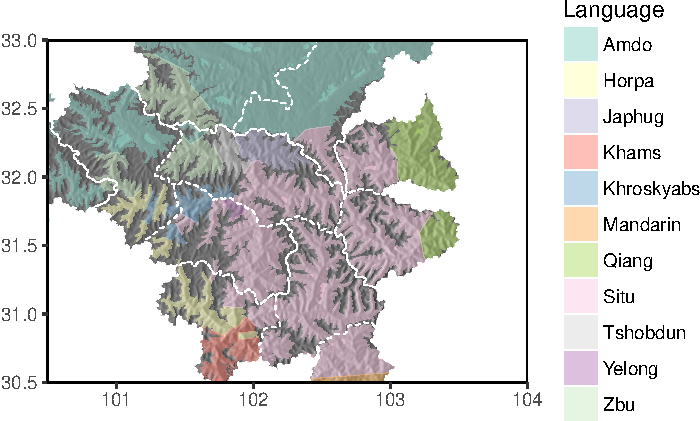
\includegraphics[width=\textwidth]{carte3.pdf}
\end{figure}

Core Gyalrong and West Gyalrongic form the Gyalrongic group \citep{jackson00puxi}, itself a subbranch of Burmo-Gyalrongic (\citealt{jacques.michaud11naish}) and possibly  the larger Tibeto-Gyalrongic group \citep{Sagart19ST}.

Japhug is in contact with both Standard Mandarin and a local variety of Sichuanese. Since no study has focused on the Sichuan Mandarin as spoken by Gyalrong speakers in Mbarkham, the present work represents all Chinese words in Standard Mandarin and pinyin (between chevrons), except for highly nativized Chinese words, presented in IPA.

Situ Gyalrong and Amdo Tibetan used to be the two dominant languages in the area, and many speakers of Japhug also have a passive understanding of Situ, and sometimes also of Tshobdun and Zbu.\footnote{See for example \ref{ex:nW.mACtsxa} (§\ref{sec:terminative}), \ref{ex:nWlWz.thWkWGe.tsa} (§\ref{sec:relative.postverbal}) and \ref{ex:mAkABzu.mWjkHW} (§\ref{sec:ra.khW.jAG.verb}), where Tshendzin recounts her experience as a teacher in Tshobdun village, where she had to learn Tshobdun to make herself understood by the pupil's parents. }


 
 \section{The Japhug corpus}
With the exception of a chapter in \citet[468--486]{linxr93jiarong} on phonology and a few articles by Lin Youjing (\citealt{linluo03, lin11direction}) (all on the Tatshi dialect), the available data on Japhug
are essentially from my own fieldwork, based on nine trips (July-August 2002, April-July 2003, July-August 2005, July 2010, July-August 2012, April-May 2014, July-August 2015, July-August 2016, May 2018) and constant contact by phone with my main language consultants. Some texts have been recorded with the help of my former PhD students Gong Xun and Lai Yunfan.
 
A short grammar \citep{jacques08}, some texts \citep{jacques10gesar}, a dictionary \citep{jacques15japhug} have previously been made available, to which a corpus of transcribed stories on the  Pangloss archive \citep{michailovsky14pangloss} can be added, available on \url{https://lacito.vjf.cnrs.fr/pangloss/corpus/list_rsc.php?lg=Japhug&name=japhug}.


My main consultant is Tshendzin (Chenzhen \zh{陈珍}, female, born 1950), a retired schoolteacher (a native speaker of Japhug, bilingual in Sichuan Mandarin since childhood), whose speech and grammaticality judgements are taken as the norm of this grammar. 

Stories  have also been collected from her husband \forme{χpɤltɕin} Dpalcan \zh{柏尔青}, her maternal uncle Andzin, her nephew (sister's child) Ayang/Kunbzang 'Tsho, and other Kamnyu people, in particular  Tshering Skyid. Most traditional stories are typical of Tibetan folklore and not specific to Japhug-speaking areas, but some procedural texts, description of local plants and animals, as well as accounts of local topography, include unique insight on local culture. In addition, a few conversations have been recorded.
 
The majority of examples in this grammar (except in the grammar sketch in chapter \ref{chap:sketch}) are taken from texts or conversations rather than elicited. Most of the texts cited are already available on Pangloss, and the examples are cited using a title in ASCII characters followed by a line number.\footnote{ \citet[305]{hill17statest} reports that this citation format is sufficient to find the relevant data. } Conversations are not included in the archive at the moment of writing, but individual sound files of the sentences quoted in this grammar are preserved in a private database. In addition, a certain amount of sentences have been noted down during participant observation, and lack recordings.
 
Since speakers I have worked with only recount a limited number of traditional stories (some of which in any case are from written sources; in particular, one of the stories told by Kunbzang Mtsho is clearly adapted from a Grimm story), I have resorted to translation from Chinese to collect a larger corpus. Tshendzin provided surprisingly idiomatic renderings of various storybooks for children (including Grimm tales, Andersen tales, Liaozhai zhiyi \zh{聊斋志异}, Arabian nights and Xiyouji \zh{西游记}). These documents are not given the same value as more spontaneous texts, and are systematically indicated  by adding the extension ``-zh" to the document name. Systematic comparison with the original text is offered whenever any suspicion of calque from Chinese exists. However, the immense morphosyntactic difference between Chinese and Japhug makes it necessary to completely rework the structure of the sentences in most cases (see for instance \ref{ex:CWmaqʰua}, §\ref{sec:apprehensive.function}), so that even if there is undoubtedly influence from Chinese, even the way Chinese is adapted into Japhug is itself an interesting topic of research.



\section{Structure of the grammar}
Rather than being intended as the final word on Japhug grammar, this book is conceived as a tool for exploring  the Japhug corpus and learning the language. 

The reader is invited to start with the grammar sketch (chapter \ref{chap:sketch}). The rest of the grammar contains two chapters on phonology (\ref{chap:phono}, §\ref{sec:clusters.redp}), five on nouns and noun phrases (\ref{chap:nominal.morphology} to \ref{chap:noun.phrase}), eleven on verbal morphology (\ref{chap:verb.template} to \ref{chap:tame}), five on syntax (§\ref{sec:basic.syntax} to \ref{chap:degree}), as well as a chapter \ref{chap:ideophones.sfp} on expressives and another one \ref{chap:kinship} on kinship.

In writing this grammar I have always preferred to abstain from definite judgement rather than provide incorrect data, and the description remains thus incomplete in many aspects, in particular in accounting for minute semantic differences between similar constructions, or on the grammaticality of borderline sentences (about which speakers sometimes change their mind). There are many points of uncertainty in many aspects of the morphosyntax (and even in some topics of phonology), and further research on finer points of phonology, morphosyntax and historical linguistics are much needed, with additional data from different speakers.

\section{Language and culture}
This work focuses on the grammar of the language, and only contains a single chapter (\ref{chap:kinship}, on the kinship system) dedicated to ethnology. However, the corpus that has been collected contains many traditional stories, as well as procedural texts describing the traditional life before massive sinicization. Examples from these texts are found on nearly all the pages of this grammar, and their interest is not purely linguistic. Thus, the section on place names presents a mythological story explaining the origin of a name (\ref{ex:qaprANar.kW}, §\ref{sec:place.names}), the chapter on orientation preverbs contains an account of the traditional living-room/kitchen (§\ref{sec:orientation.kitchen}) and an introduction to weaving (§\ref{sec:orientation.loom}), and the section on antipassive derivations includes a passage on rain-calling and mountain tutelary spirits  (see example \ref{ex:znArGAma}, §\ref{sec:antipassive.avoidance}). In this sense, traditional culture permeates this grammar from beginning till end.

Further ethnographical work is necessary, in particular on kinship \citep{zhangsy20kinship}, traditional houses \citep{dongsy18chabao}, weaving and ethnobotany, and it is hoped that this grammar (together with the dictionary) will make it possible to properly describe local culture through the medium of Japhug rather than Chinese.

